\documentclass[10pt,twocolumn,letterpaper]{article}

\usepackage{cvpr}
\usepackage{times}
\usepackage{epsfig}
\usepackage{graphicx}
\usepackage{amsmath}
\usepackage{amssymb}
\usepackage[usenames,dvipsnames]{color}
\usepackage{color}
\usepackage{etoolbox}
\usepackage{listings}
\usepackage{mathtools}
\usepackage{subcaption}
\usepackage{verbatim}
\robustify{\cite}


\definecolor{todo-color}{rgb}{1,0,0}
\newcommand{\todo}[1]{\textnormal{\color{todo-color}{\textbf{#1}}}\unskip}

% Include other packages here, before hyperref.

% If you comment hyperref and then uncomment it, you should delete
% egpaper.aux before re-running latex.  (Or just hit 'q' on the first latex
% run, let it finish, and you should be clear).
\usepackage[breaklinks=true,bookmarks=false]{hyperref}

\cvprfinalcopy % *** Uncomment this line for the final submission

\def\cvprPaperID{****} % *** Enter the CVPR Paper ID here
\def\httilde{\mbox{\tt\raisebox{-.5ex}{\symbol{126}}}}

% Pages are numbered in submission mode, and unnumbered in camera-ready
%\ifcvprfinal\pagestyle{empty}\fi
%\setcounter{page}{4321}
\begin{document}

%%%%%%%%% TITLE
\title{Miniplaces Project Report - Team ``deepkuso''}

\author{Matthew Perron\\
MIT CSAIL\\
{\tt\small mperron@mit.edu}
% For a paper whose authors are all at the same institution,
% omit the following lines up until the closing ``}''.
% Additional authors and addresses can be added with ``\and'',
% just like the second author.
% To save space, use either the email address or home page, not both
\and
Joana M. F. da Trindade\\
MIT CSAIL\\
{\tt\small jfon@mit.edu}
}

\maketitle
%\thispagestyle{empty}

%\begin{abstract}
%\end{abstract}

\section{Introduction}

We describe our approach to designing an image classification algorithm for the Miniplaces challenge. At a high level our approach is an ensemble of a small number of deep networks. We describe our choice of deep network architectures, and our ensembling technique in detail. 
\section{Approach}

We took three approaches to improve the performance of our model against the baseline Alexnet~\cite{alexnet} model trained with the example code. First, we trained newer, smaller, network architectures on the training set including Inception~\cite{inception} and ResNet~\cite{resnet}. Second, we augmented our training data to reduce overfitting during training by altering the image properties (color, brightness, etc), taking a random sub-image, and flipping the image vertically. Finally, we ensembled our best performing models together with a range of techniques described in detail in Section~\ref{s:experiments}. Using these three methods together yielded the best results on our validation set.

\subsection{Network Architectures}
With the baseline AlexNet code, we were able to achieve about 70\% top-5 accuracy. We felt that with newer model architectures, it would be possible to achieve higher performance. We settled on two models, ResNet V2 101 and Inception V3. Even with fewer parameters these architectures are shown to perform better on the Imagenet~\cite{imagenet} classification task~\cite{model-comparison}. We reasoned that these architectures may also perform well on the Miniplaces task compared to AlexNet without a significant impact on training time. Inception is a deep network architecture made up of many stacked inception modules, as seen in Figure \ref{fig:inception-module}. Inception allows for the expressibility of some 5x5 convolutions without forcing the entire layer to consist of these large convolutions, this saves parameters without giving up expressibility. We also trained a ResNet model. ResNet forwards the output of some layers forward in the network, and adds them together. Effectively this means that during backpropagation the gradients from some subsections of the network can be passed back to earlier layers of the network without going through intermediate layers. This can be seen in the ResNet block in Figure \ref{fig:resnet-block}. Another advantage of both Inception V3 and Resnet is a single fully connected layer compared to AlexNet's two, reducing the number of parameters required. We trained these networks with standard batch normalization and dropout techniques. 

\begin{figure}[b]
\centering
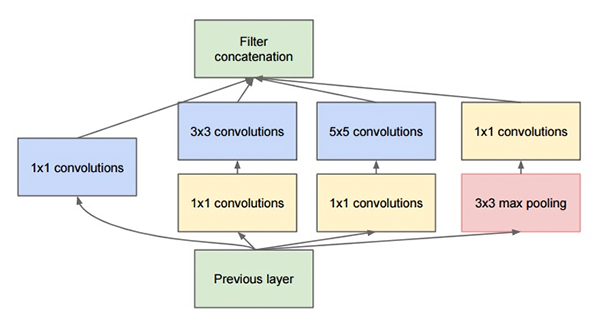
\includegraphics[width=\columnwidth]{figures/inception_module}
\caption{Single Inception~\cite{inception} module}
\label{fig:inception-module}
\end{figure}

\begin{figure}[b]
\centering
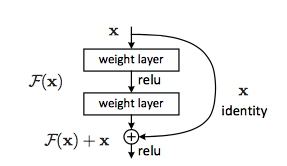
\includegraphics[width=\columnwidth]{figures/residual_block}
\caption{Single Resnet~\cite{resnet} block}
\label{fig:resnet-block}
\end{figure}

\subsection{Data Augmentation}
In the course of training our models, we found that many of the models overfit our training data, achieving near perfect top-1 accuracy on the the training set, but had 10s of percentage points worse accuracy on the validation set. We reasoned that the model was 'memorizing' the training set and not generalizing well. Even at best, the models accuracy on the validation set was around 70\%.We augmented our dataset using four techniques; perturbing image properties, mirroring the image, and taking a random subimage. Each of these operations is performed randomly at training time by taking an image and perturbing it with a random order of the above techniques before passing into the network. All of these operations are part of the input pipeline during training time. Thus we do not explicitly create new examples, but generate them on the fly during training. In this way we virtually increase the number of training samples and are more robust to overfitting. 

We first augment the color of the image by perturbing image-wide properties including  brightness, saturation, hue, and contrast by a random amount. We are careful to choose only perturbations that output images recognizably in the same class as the original image. We shuffle the order of these operations for each input image since the perturbations do not commute. This, we reason, prevents the network from learning pixel patterns in the image by slightly changing the training images on each batch and should generalize better than a network without this augmentation to the input. 

We also kept the augmentation techniques present in the Tensorflow example code, namely flipping the image along its horizontal axis at random, and taking a random crop of the image.

\subsection{Ensembling Techniques}

Ensemble learning techniques combine multiple trained baseline models to make the final set of predictions.  In traditional machine learning, ensemble methods are mainly divided in three categories: bagging, boosting, and stacking \cite{ensembleML2012}.  With bagging, the final prediction is obtained as a weighted majority over predictions from each baseline model.  In boosting, each model specializes on certain subsets of examples.  Finally, stacking ensembles use the prediction of each baseline model to train a new model which outputs a combined prediction.

\subsection{Bagging Ensemble Of CNNs}
\label{ss:ensembling}

In our solution we opted for using bagging as the ensemble method, and grid search to explore the search space of model weights and other hyperparameter values. We considered ensembling all the models by removing their respective final fully connected layers and fine-tuning all networks with a shared fully connected layer (or otherwise a ``stacking'' ensemble, as described in Section~\ref{ss:ensembling}). However, limitations on GPU memory made this approach difficult. So we decided on a simpler bagging approach.

One technique we consider in our grid search takes into account the class-wise accuracy or class-wise confidence calculated on the training set for each model. The class-wise accuracy is given by $\frac{\textbf{true positives}}{\textbf{ \# class examples}}$. the class-wise confidence is given by $\frac{\textbf{true positives}}{\textbf{ true positives + false positives}}$. For each model, on each class we calculated it's accuracy and confidence for its top-1 and top-5 guesses. We the weigh the output of each network based on its accuracy or confidence in guessing examples on the validation set.
\section{Experiments}
\label{s:experiments}

The AlexNet models were trained on a desktop with an 8 core Intel(R) Core(TM) i7-6900K CPU @ 3.20GHz CPU and a Nvidia Titan-X GPU with 12GB of onboard memory. 

The Inception and Resnet models were trained on a server with two 22-core Intel(R) Xeon(R) CPU E5-2699 v4 @ 2.20GHz CPUs and a Tesla P100 GPU with 16GB of onboard memory.

We trained both our Inception-V3 and ResNet-V2-101 models using the Tensorflow~\cite{tensorflow} Slim framework. We trained our AlexNet models by modifying the example code. All models were trained with an Adam Optimizer~\cite{adam}. For Inception and ResNet our best models trained with $0.8$ keep probability for dropout, an initial learning rate of $0.1$, and optimizer parameters $\beta_1 = 0.9$ and $\beta_2 =0.999$. The learning rate was decayed every 25 batches. We used a batch size of 128 for ImageNet and 60 for ResNet. Otherwise the initialization for Inception V3 is identical to the Inception~\cite{inception} Paper. Our best AlexNet model was trained with a  $0.5$ keep probability for dropout and an initial learning rate of $0.001$ and the Tensorflow default parameters for the Adam optimizer.

%% subsection: Grid Search
\begin{table*}[!htb]
\small
\centering
 \begin{tabular}{|p{7cm}|p{3cm}|p{1.5cm}|p{1.5cm}|}
 \hline
Model weights & Decay type & Top-1 Acc & Top-5 Acc\\\hline\hline
alexnet: 1.0,
inception: 1.0
resnet: 1.0 & exponential & 0.5323 & 0.8203 \\\hline
alexnet: 0.7,
inception: 1.0,
resnet: 1.0 & exponential & 0.5318 & 0.8177 \\\hline
alexnet: 0.7,
inception: 0.7,
resnet: 1.0 & exponential & 0.531 & 0.8177 \\\hline
alexnet: 0.7,
inception: 1.0,
resnet: 0.7 & exponential & 0.5268 & 0.8169 \\\hline
alexnet: 0.7,
inception: 1.0,
resnet: 1.0 & linear & 0.5202 & 0.8165 \\\hline
alexnet: 1.0,
inception: 1.0,
resnet: 0.7 & exponential & 0.5282 & 0.8151 \\\hline
alexnet: 0.7,
inception: 1.0,
resnet: 0.7 & linear & 0.5191 & 0.8142 \\\hline
alexnet: 1.0,
inception: 0.7,
resnet: 1.0 & exponential & 0.5199 & 0.8141 \\\hline
alexnet: 1.0,
inception: 1.0,
resnet: 1.0 & linear & 0.5218 & 0.8140 \\\hline
alexnet: 1.0,
inception: 0.7,
resnet: 0.7 & linear & 0.5279 & 0.8136 \\\hline
\end{tabular}
\caption{Top 10 bagging ensemble configurations, as ranked by top-5 accuracy over validation set.}
\label{tab:top10_configs}
\end{table*}

\subsection{Grid Search Hyperparameters}

We use grid search to explore the space of hyperparameter values that yield the best top-5 accuracy over validation set. Hyperparameters on the search space are:\\

\noindent {\bf Model weights.} We define a 'model weight' as the weight for each model in the weighted majority bagging ensemble prediction. This value ranges from 0.0 to 1.0 for each model.  After initially experimenting with varying model contributions in increments of 0.25, we found no gains in validation accuracy for any configuration where weight was less than 0.7.  Therefore, for our final grid search we use either 0.0, 0.7 or 1.0 as the weight for each model in the bagging ensemble.\\

\noindent {\bf Decay function.} We define 'decay function' as the function over the prediction ranks of each model. We consider three different decay functions:

$$\text{Constant: } D(r,k) \begin{cases}
               1.0 \text{ if } r < k\\
               0.0 \text{ otherwise}
            \end{cases}$$

$$\text{Linear: } D(r) = |\text{prediction\_classes}| - r$$

$$\text{Exponential: } D(r) = e^{\frac{-r}{5}}$$
 
where $r$ is the prediction rank and in the case of ``Constant'', $k$ is a rank cutoff, e.g., $k = 5$ if only the first 5 predictions of that model are considered for the weighted majority vote.  We use two variations of constant decay function, one where $k = 5$, and another where $k = 10$. In our experiments, we find that the best results are obtained when the decay function is either exponential, or constant with $k = 5$.\\

\noindent {\bf Class-wise confidence.} As described in Section~\ref{ss:ensembling}, we also consider an heuristic that takes into account the class-wise confidence as calculated over the training set.  This adds a total of four permutations per configuration, as both top-1 and top-5 class-wise confidence is considered.\\

\noindent {\bf Class-wise accuracy.} The final heuristic we include as part of the grid search space is class-wise accuracy, defined in Section~\ref{ss:ensembling}.  Similar to class-wise confidence, this hyperparameter too adds four permutations per configuration to the total search space we explore with grid search.\\

An example configuration for the grid search space, together with its top-1 and top-5 accuracy over validation set is given in Figure ~\ref{fig:gs_config}.  In Table~\ref{tab:top10_configs} we display the 10 best configurations found by our grid search over the hyperparameters described above. Other configurations and their accuracies over validation set are included in the accompanying source code, under \texttt{weighted\_majority/grid\_search\_results.txt}.

\subsection{Ensemble Weight}

The ensemble value of a single class prediction for an image is given by the formula:

$$E(p,r) = \sum_{n=1}^{|models|} w_n * c_p * a_p * d(r)$$

where $p$ is the prediction class, $r$ is the rank of that class as given by CNN model $n$, $w_n$ is the weight (for majority vote) assigned to that model, $c_p$ is the class-wise confidence score for prediction class $p$, $a_p$ is the class-wise accuracy for prediction class $p$, and $d$ is the contribution of rank $r$ after decay function is applied.

For example, given the grid search configuration in Figure~\ref{fig:gs_config}, $c_p$ would be set to 1.0 since class-wise confidence scores are disabled, and $a_p$ would also be set to 1.0 for a similar reason. Further, $d(r)$ would be the result of applying the ``Constant'' decay function with $k = 5$, yielding 0.0 if $r > 5$, and $w_n$ would be 1.0 regardless of model (AlexNet, ResNet, or Inception).  So in this case, the final ensemble value for class $p$ is equal to the weighted majority of the three different CNNs, with equal weight assigned to each.

\begin{figure}[!ht]
\verbatiminput{grid_search_config.txt}
\caption{Example configuration explored by grid search, together with resulting top-1 and top-5 accuracy over validation set.}
\label{fig:gs_config}
\end{figure}

\subsection{Best Performing CNN Ensembles}

Table~\ref{tab:top10_configs} shows the top 10 configurations, as ranked by top-5 accuracy over validation set.  Our grid search also explores configurations where class accuracies and class confidence scores for both top-1 and top-5 -- as defined in Section~\ref{ss:ensembling} -- are considered.  We find, however, that the configurations with highest top-5 accuracy over validation set are obtained when neither of these heuristics are considered.  In addition, our experimental results indicate highest top-5 accuracy over validation set is obtained when all models have similar weights, i.e., the simple weighted majority case.
\section{Conclusion}

We find that single neural networks suffered from significant overfitting and none were able to achieve an accuracy above 77\% on the validation or test sets. We used several techniques to mitigate the drawbacks of these models including augmenting the training data with perturbations and changing the dropout keep probability to improve individual models. However even though this yielded small improvements, only ensembling techniques improved the accuracy significantly (over 80\%).

Had we more computational resources available, we would have liked to experiment with larger batch sizes, as well as stacking instead of bagging ensemble.

{\small
\bibliographystyle{ieee}
\bibliography{egbib}
}

\end{document}
